\section*{Question 8}
\fakesection{8}

\begin{enumerate}[label=\alph*)]

    \item Using fast.ai \texttt{dataloaders}, the batch size can be specified using the \texttt{bs} argument:
    \begin{center}
        \texttt{dls = DataBlock(...).dataloaders(..., bs=BATCH\_SIZE)}
    \end{center}
    Using a ResNet-18 model pre-trained on the ImageNet dataset, we compare model training speed using batch sizes of: 16, 32, 64, 128 and 256 samples. Three trials are performed for each batch size. Each trial re-initialises the model and fine-tunes it for three epochs. Table \ref{tab:bs_exp} records the average time per trial.

    \begin{table}[ht]
        \small \centering \restretch{1.2}
        \caption{Average training time for 3 epochs with varying batch size}
        \begin{tabularx}{0.33\textwidth}{c c}
            \toprule
            \textbf{Batch Size} & \textbf{Avg. Time (s)} \\
            \midrule
             16 & 7.81 \\
             32 & 6.92 \\
             64 & 6.41 \\
            128 & 5.79 \\
            256 & 5.89 \\
            \bottomrule
        \end{tabularx}
        \label{tab:bs_exp}
    \end{table}

    The tabulated data suggests that for the modest hardware on which the experiments were performed (an NVIDIA 3060 GPU), a batch size of 128 samples is most efficient, followed closely by a batch size of 256 samples. The reason for this is elaborated on in part c).

    \item We can also compare the performance of CUDA from Table \ref{tab:bs_exp} to the CPU using
    \begin{center}
        \texttt{fastai.torch\_core.default\_device(False)}
    \end{center}
    which disables CUDA as the default device (hence defaulting to the CPU). Table \ref{tab:bs_exp_cpu} repeats the experiment of part a) on the CPU with a reduced selection of batch sizes.

    \begin{table}[ht]
        \small \centering \restretch{1.2}
        \caption{Average training time for 3 epochs with varying batch size}
        \begin{tabularx}{0.48\textwidth}{c c c}
            \toprule
            \textbf{Batch Size} & \textbf{Avg. Time (s)} & \textbf{Vs. CUDA} \\
            \midrule
             16 & 115.54 & 14.79$\times$ \\
             64 & 105.70 & 16.49$\times$ \\
            256 &  98.92 & 16.79$\times$ \\
            \bottomrule
        \end{tabularx}
        \label{tab:bs_exp_cpu}
    \end{table}

    Unsurprisingly, CUDA eclipses CPU performance in all cases, approaching a factor of 17 for batch sizes of 64 and 256. CUDA leverages hardware designed for parallel compute, whereas CPUs are predominantly serial. CUDA therefore achieves significantly better machine learning performance, where a batch can be processed all at once in parallel.

\newpage

    \item Finally, we use the native Windows system monitor to compare GPU activity when fine-tuning the ResNet for three epochs using a batch size of 16 versus 128.

    \begin{figure}[ht]
        \centering
        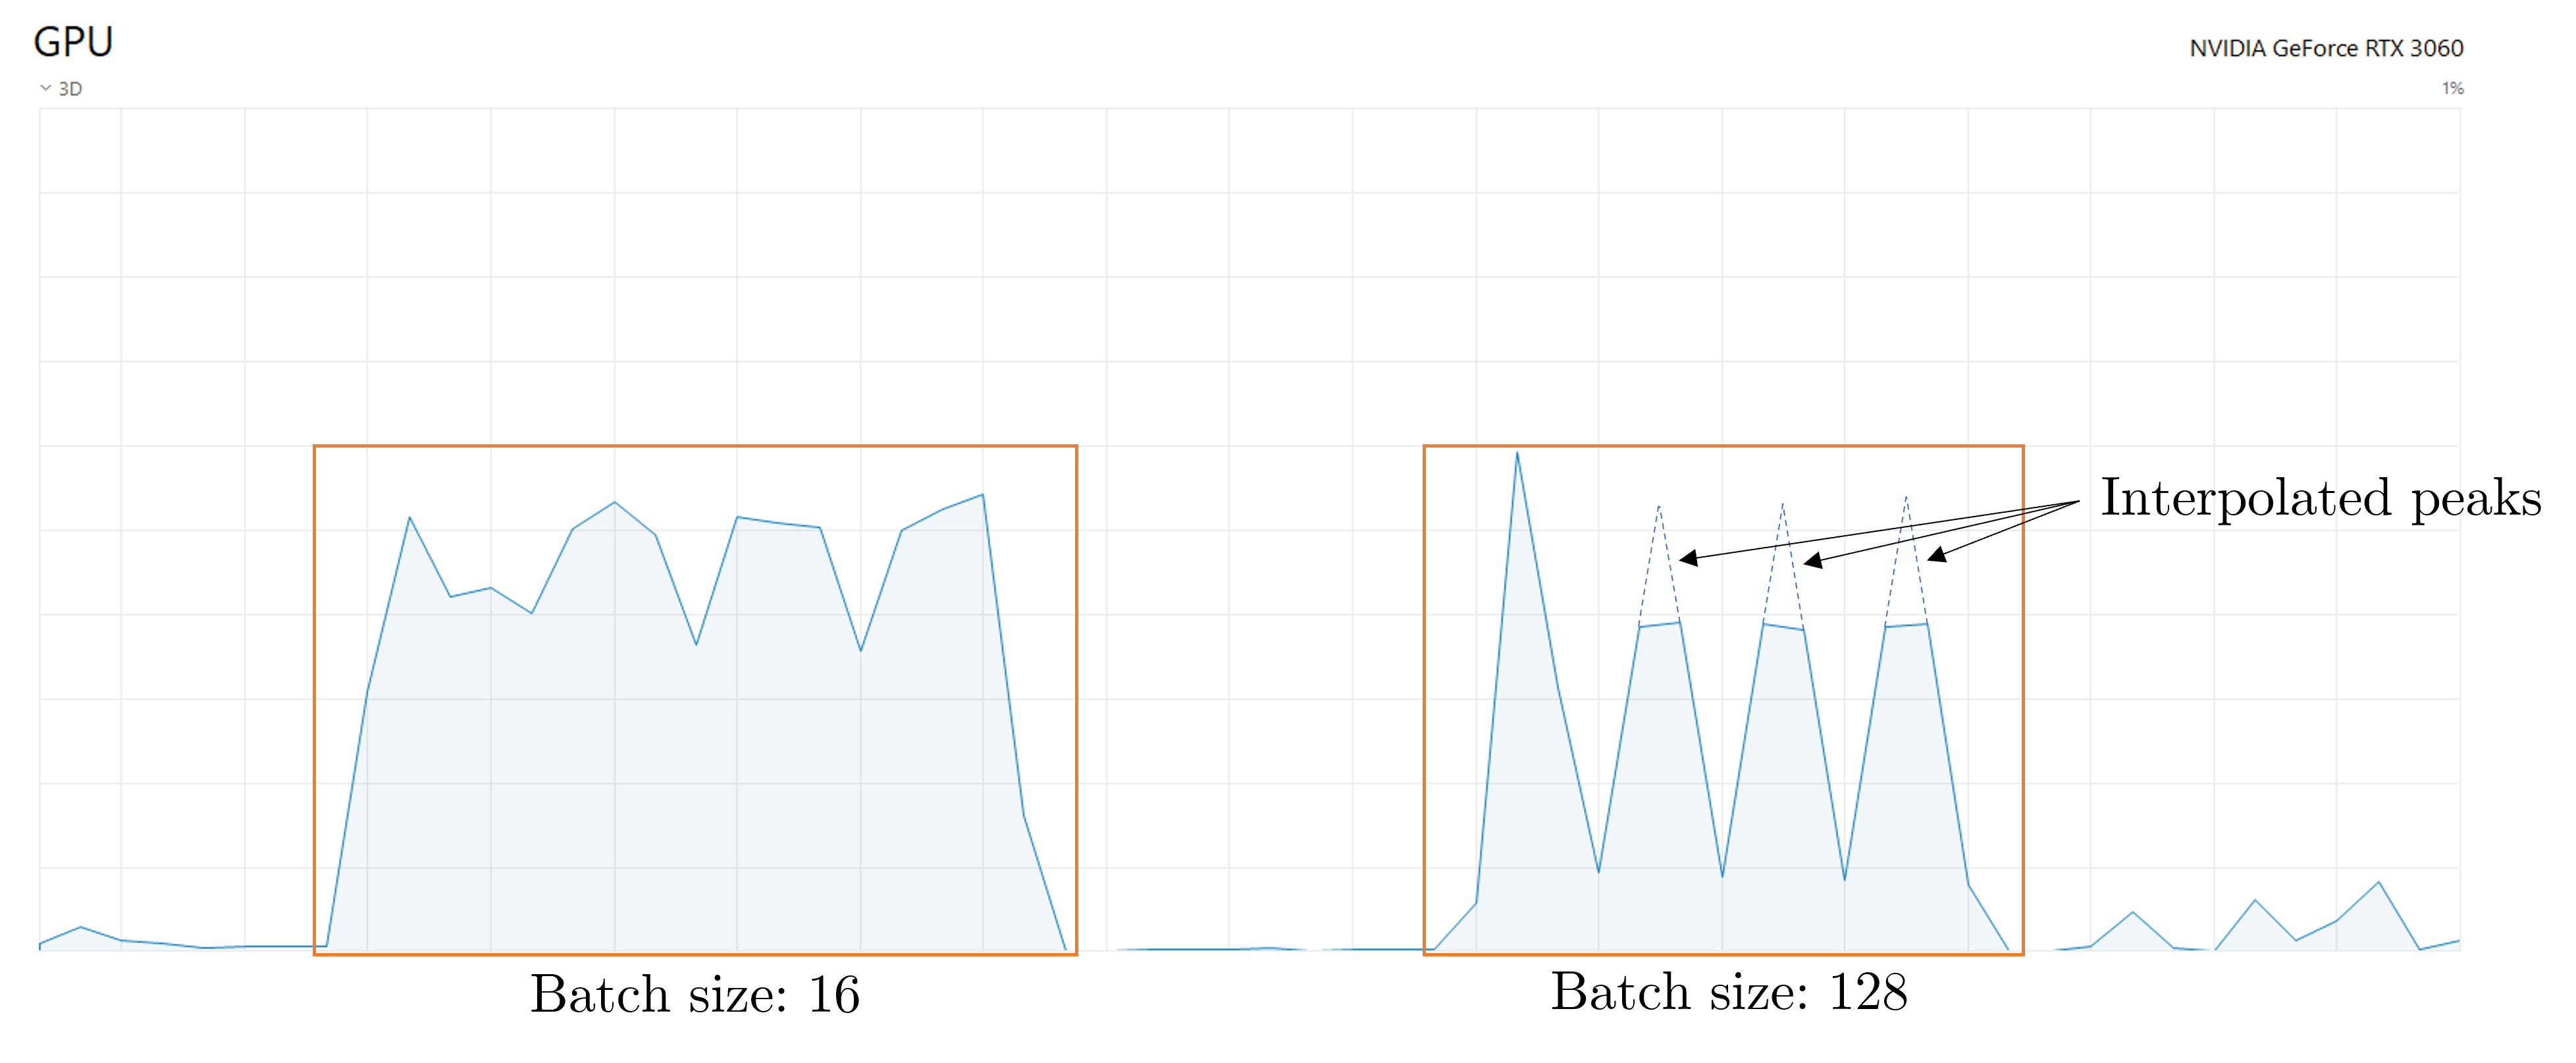
\includegraphics[width=0.9\textwidth]{images/q8_gpumon.png}
        \caption{GPU activity fine-tuning three epochs with batch sizes of 16 and 128}
        \label{fig:q8_gpumon}
    \end{figure}

    Firstly, though we specify only three epochs of fine tuning, we notice four peaks in GPU activity for both batch sizes. The default behaviour of the fast.ai \texttt{fine\_tune} method is to freeze the model (prevent parameter updates for all layers except the last few) for one epoch, then unfreeze the model and complete the specified number of epochs. Hence, four epochs are completed in total.

    We also note that, as identified in Table \ref{tab:bs_exp}, a batch size of 128 finishes faster than a batch size of 16. The peaks in activity are more pronounced for a batch size of 128. In fact, as a caveat of the maximum refresh rate of the system monitor, the activity is probably even underrepresented in Figure \ref{fig:q8_gpumon}, and probably peaks much closer to 100\% utilisation for a batch size of 128.

    As mentioned in part b), CUDA devices are highly parallel and can process entire batches simultaneously given they fit in device memory. With a batch size of 16, we do not maximise the parallel capacity of the GPU; hence, we observe wider but shorter peaks. In this case, the computation is memory-bound rather than throughput-bound. With a batch size of 128, we make much fuller use of the parallel capacity; hence, we observe narrow but taller peaks. However, if we continue to increase the batch size, we will eventually see no improvement in performance. This occurs when we have the maximum batch size that fits into GPU memory, at which point the computation becomes throughput-bound.

\end{enumerate}
